\clearpage
\subsection{Fast Simulation vs Detector Emulation} \label{sec::App::valid_smear}
In order to save the computing resources, only a few signal models are generated with detector simulation ($\checkmark$ in Table \ref{tab::Introduction::modelsBV}-\ref{tab::Introduction::models3B}).
The detector response for the samples of the other models are then emulated, using the parametrized efficiency functions (in terms of electron identification, muon identification, isolation cut, JVT cut and $b$-tagging) and smearing fucntions (in terms of energy resolution of objects and $\met$) from full-simulated $\ttbar$ samples. 
The emulation is validated by comparing the kinematics of signals with the samepls of fast-simulation.
3 reference mass points for \textbf{QQC1QQC1} and one reference point for \textbf{TTN1TTN1} are chosen, and results are shown in Figure \ref{fig::Samples::valid_smear_GG_symQQC1_2000_1000_1}-\ref{fig::Samples::valid_smear_GG_symTTN1_2000_5000_400}. 
In the bulk phase space, the difference is within $10\%$ which is sufficient with respect to the signal cross-section uncertainty ($15\%\sim35\%$).
The emulation is sometimes not perfect in the tail of the distributions, however it does not matter for most of the cases since such region does not address any signal sensitivity. 

 %%%%%%%%%%%%%%%%%%%%%%%%%%
\begin{figure}[h]
  \centering
    \subfig{0.23}{figures/Samples/valid_smear/GG_symQQC1_2000_1000_1/plot/nJet__1LMET200.pdf}{Jet multiplicity}
    \subfig{0.23}{figures/Samples/valid_smear/GG_symQQC1_2000_1000_1/plot/jet1Pt__1LMET200.pdf}{$\pt$ of the leading jet}
    \subfig{0.23}{figures/Samples/valid_smear/GG_symQQC1_2000_1000_1/plot/meffInc30__1LMET200.pdf}{$\meffInc$}
    \subfig{0.23}{figures/Samples/valid_smear/GG_symQQC1_2000_1000_1/plot/lep1Pt__1LMET200.pdf}{$\pt$ of the leading lepton}
    \subfig{0.23}{figures/Samples/valid_smear/GG_symQQC1_2000_1000_1/plot/met__1LMET200.pdf}{$\met$}
    \subfig{0.23}{figures/Samples/valid_smear/GG_symQQC1_2000_1000_1/plot/mt__1LMET200.pdf}{$\mt$}
    \subfig{0.23}{figures/Samples/valid_smear/GG_symQQC1_2000_1000_1/plot/metOverMeff__1LMET200.pdf}{$\met/\meffInc$}
    \subfig{0.23}{figures/Samples/valid_smear/GG_symQQC1_2000_1000_1/plot/LepAplanarity__1LMET200.pdf}{Aplanarity}
    \subfig{0.6}{figures/Samples/valid_smear/GG_symQQC1_2000_1000_1/plot/regionYields__SRsBV.pdf}{Yields in b-vetoed signal regions}
    \caption{
        \textbf{QQC1QQC1},  $(\mG,\mC,\mN) = (2000,1000,0) \gev$
   }
   \label{fig::Samples::valid_smear_GG_symQQC1_2000_1000_1} 
\end{figure}
 %%%%%%%%%%%%%%%%%%%%%%%%%%

\clearpage
 %%%%%%%%%%%%%%%%%%%%%%%%%%
\begin{figure}[h]
  \centering
    \subfig{0.28}{figures/Samples/valid_smear/GG_symQQC1_1700_1500_60/plot/nJet__1LMET200.pdf}{Jet multiplicity}
    \subfig{0.28}{figures/Samples/valid_smear/GG_symQQC1_1700_1500_60/plot/jet1Pt__1LMET200.pdf}{$\pt$ of the leading jet}
    \subfig{0.28}{figures/Samples/valid_smear/GG_symQQC1_1700_1500_60/plot/meffInc30__1LMET200.pdf}{$\meffInc$}
    \subfig{0.28}{figures/Samples/valid_smear/GG_symQQC1_1700_1500_60/plot/lep1Pt__1LMET200.pdf}{$\pt$ of the leading lepton}
    \subfig{0.28}{figures/Samples/valid_smear/GG_symQQC1_1700_1500_60/plot/met__1LMET200.pdf}{$\met$}
    \subfig{0.28}{figures/Samples/valid_smear/GG_symQQC1_1700_1500_60/plot/mt__1LMET200.pdf}{$\mt$}
    \subfig{0.28}{figures/Samples/valid_smear/GG_symQQC1_1700_1500_60/plot/metOverMeff__1LMET200.pdf}{$\met/\meffInc$}
    \subfig{0.28}{figures/Samples/valid_smear/GG_symQQC1_1700_1500_60/plot/LepAplanarity__1LMET200.pdf}{Aplanarity}
    \subfig{0.65}{figures/Samples/valid_smear/GG_symQQC1_1700_1500_60/plot/regionYields__SRsBV.pdf}{Yields in b-vetoed signal regions}
    \caption{ 
        \textbf{QQC1QQC1},  $(\mG,\mC,\mN) = (1700,1500,60) \gev$
    }
  \label{fig::Samples::valid_smear_GG_symQQC1_1700_1500_60} 
\end{figure}
 %%%%%%%%%%%%%%%%%%%%%%%%%%

\clearpage
 %%%%%%%%%%%%%%%%%%%%%%%%%%
\begin{figure}[h]
  \centering
    \subfig{0.28}{figures/Samples/valid_smear/GG_symQQC1_1700_260_60/plot/nJet__1LMET200.pdf}{Jet multiplicity}
    \subfig{0.28}{figures/Samples/valid_smear/GG_symQQC1_1700_260_60/plot/jet1Pt__1LMET200.pdf}{$\pt$ of the leading jet}
    \subfig{0.28}{figures/Samples/valid_smear/GG_symQQC1_1700_260_60/plot/meffInc30__1LMET200.pdf}{$\meffInc$}
    \subfig{0.28}{figures/Samples/valid_smear/GG_symQQC1_1700_260_60/plot/lep1Pt__1LMET200.pdf}{$\pt$ of the leading lepton}
    \subfig{0.28}{figures/Samples/valid_smear/GG_symQQC1_1700_260_60/plot/met__1LMET200.pdf}{$\met$}
    \subfig{0.28}{figures/Samples/valid_smear/GG_symQQC1_1700_260_60/plot/mt__1LMET200.pdf}{$\mt$}
    \subfig{0.28}{figures/Samples/valid_smear/GG_symQQC1_1700_260_60/plot/metOverMeff__1LMET200.pdf}{$\met/\meffInc$}
    \subfig{0.28}{figures/Samples/valid_smear/GG_symQQC1_1700_260_60/plot/LepAplanarity__1LMET200.pdf}{Aplanarity}
    \subfig{0.65}{figures/Samples/valid_smear/GG_symQQC1_1700_260_60/plot/regionYields__SRsBV.pdf}{Yields in b-vetoed signal regions}
    \caption{ 
    \textbf{QQC1QQC1},  $(\mG,\mC,\mN) = (1700,260,60) \gev$
    }
  \label{fig::Samples::valid_smear_GG_symQQC1_1700_260_60} 
\end{figure}
 %%%%%%%%%%%%%%%%%%%%%%%%%%

\clearpage
 %%%%%%%%%%%%%%%%%%%%%%%%%%
\begin{figure}[h]
  \centering
    \subfig{0.28}{figures/Samples/valid_smear/GG_symTTN1_2000_5000_400/plot/nBJet__1LMET200.pdf}{$b$-jet multiplicity}
    \subfig{0.28}{figures/Samples/valid_smear/GG_symTTN1_2000_5000_400/plot/nJet__1L3BMET200.pdf}{Jet multiplicity}
%    \subfig{0.28}{figures/Samples/valid_smear/GG_symTTN1_2000_5000_400/plot/jet1Pt__1L3BMET200.pdf}{$\pt$ of the leading jet}
    \subfig{0.28}{figures/Samples/valid_smear/GG_symTTN1_2000_5000_400/plot/meffInc30__1L3BMET200.pdf}{$\meffInc$}
    \subfig{0.28}{figures/Samples/valid_smear/GG_symTTN1_2000_5000_400/plot/met__1L3BMET200.pdf}{$\met$}
    \subfig{0.28}{figures/Samples/valid_smear/GG_symTTN1_2000_5000_400/plot/mt__1L3BMET200.pdf}{$\mt$}
    \subfig{0.28}{figures/Samples/valid_smear/GG_symTTN1_2000_5000_400/plot/LepAplanarity__1L3BMET200.pdf}{Aplanarity}
    \subfig{0.28}{figures/Samples/valid_smear/GG_symTTN1_2000_5000_400/plot/min_dPhi_4j__1L3BMET200.pdf}{$\mindPhiFourJet$}
    \subfig{0.28}{figures/Samples/valid_smear/GG_symTTN1_2000_5000_400/plot/topNess__1L3BMET200.pdf}{$\met/\meffInc$}
    \subfig{0.65}{figures/Samples/valid_smear/GG_symTTN1_2000_5000_400/plot/regionYields__SRsBT.pdf}{Yields in b-tagged signal regions}
    \caption{ 
        \textbf{TTN1TTN1},  $(\mG,\mN) = (2000,400) \gev$
    }   
    \label{fig::Samples::valid_smear_GG_symTTN1_2000_5000_400}
\end{figure}
 %%%%%%%%%%%%%%%%%%%%%%%%%%




%\clearpage
%\paragraph{Combined Test of Missing Lepton Replacement and Tau Replacement} \mbox{} \\
%%%%%% METHNAME %%%%%%%%%%%%%%%%%%%%%%%%%%
\begin{figure}[h]
  \centering
    \subfigure[]{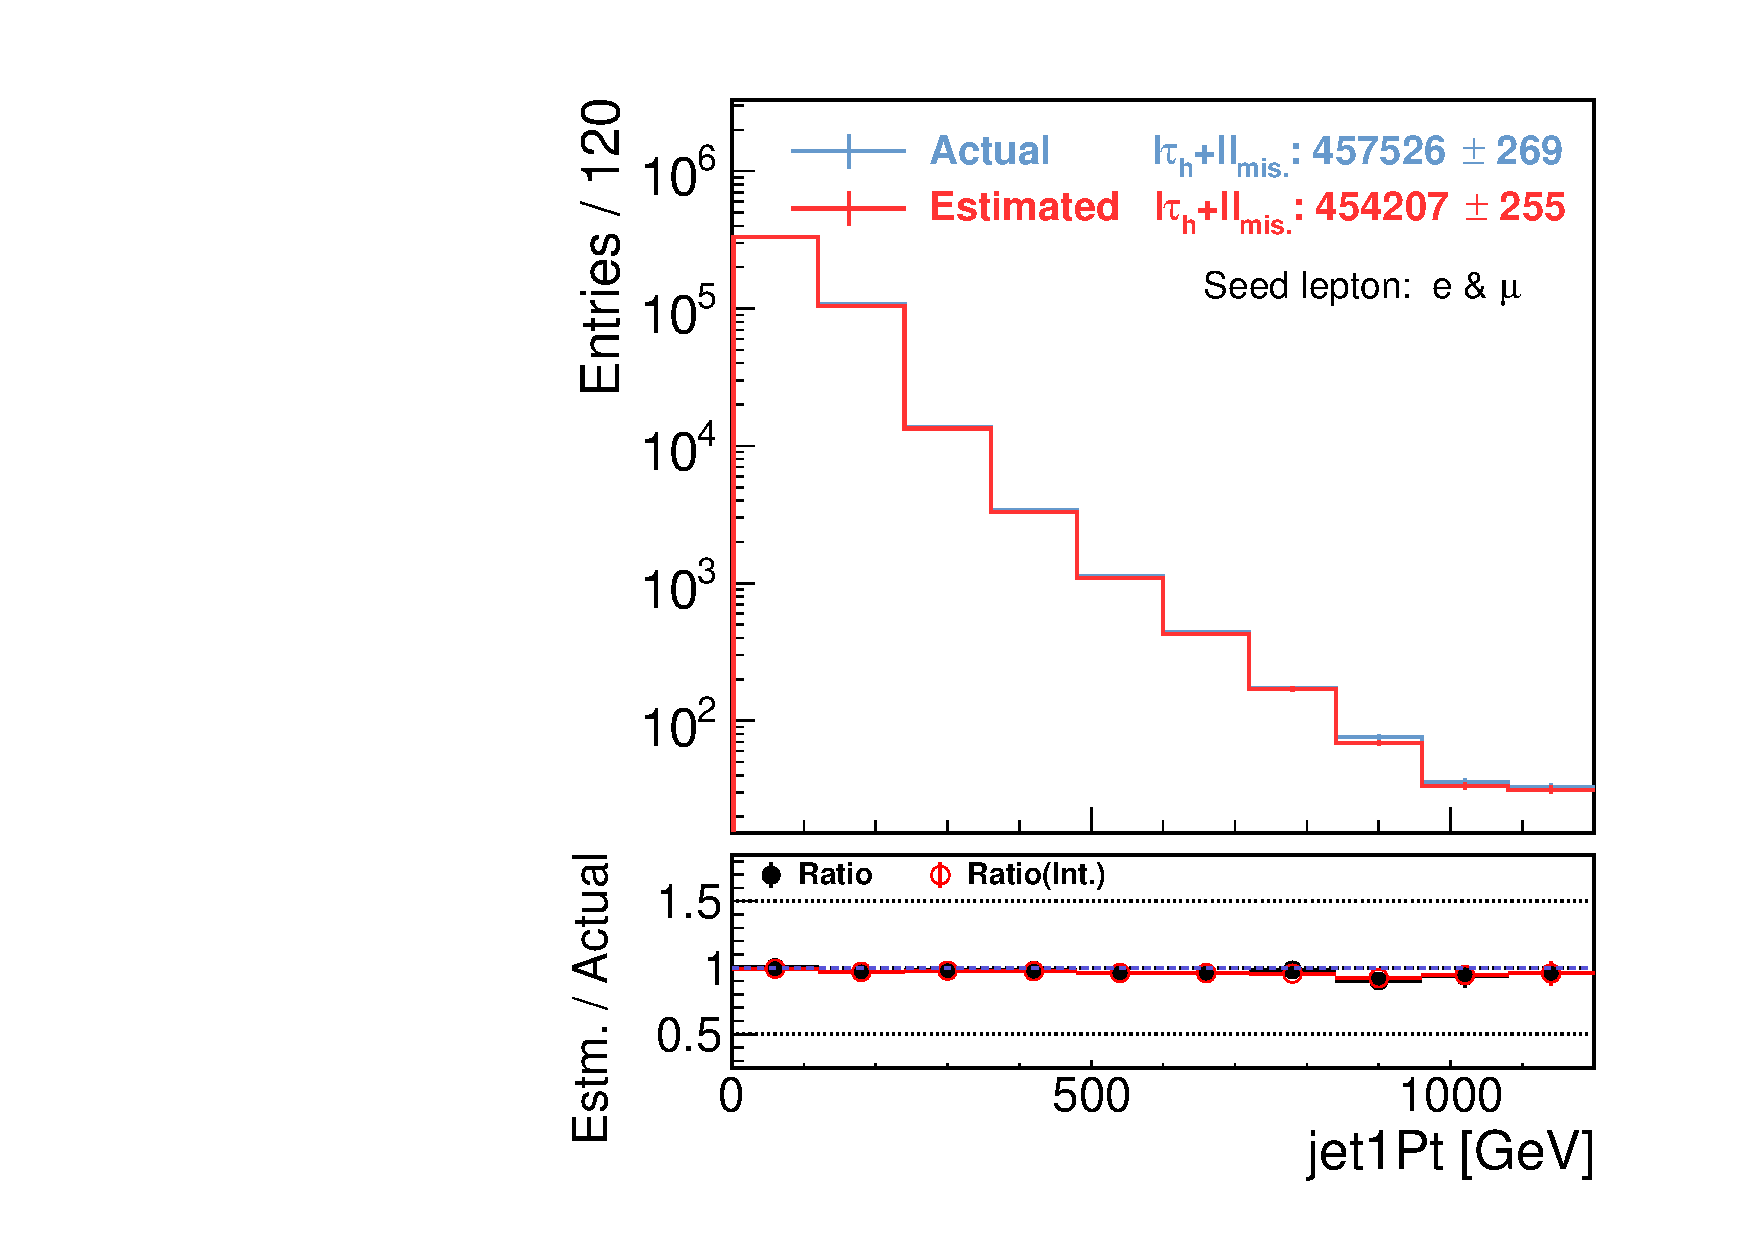
\includegraphics[width=0.32\textwidth]{figures/BGestimation/ObjReplacement/mcClosure/All_emu/All_emu_jet1Pt__trMode4_NoSys.pdf}}
    \subfigure[]{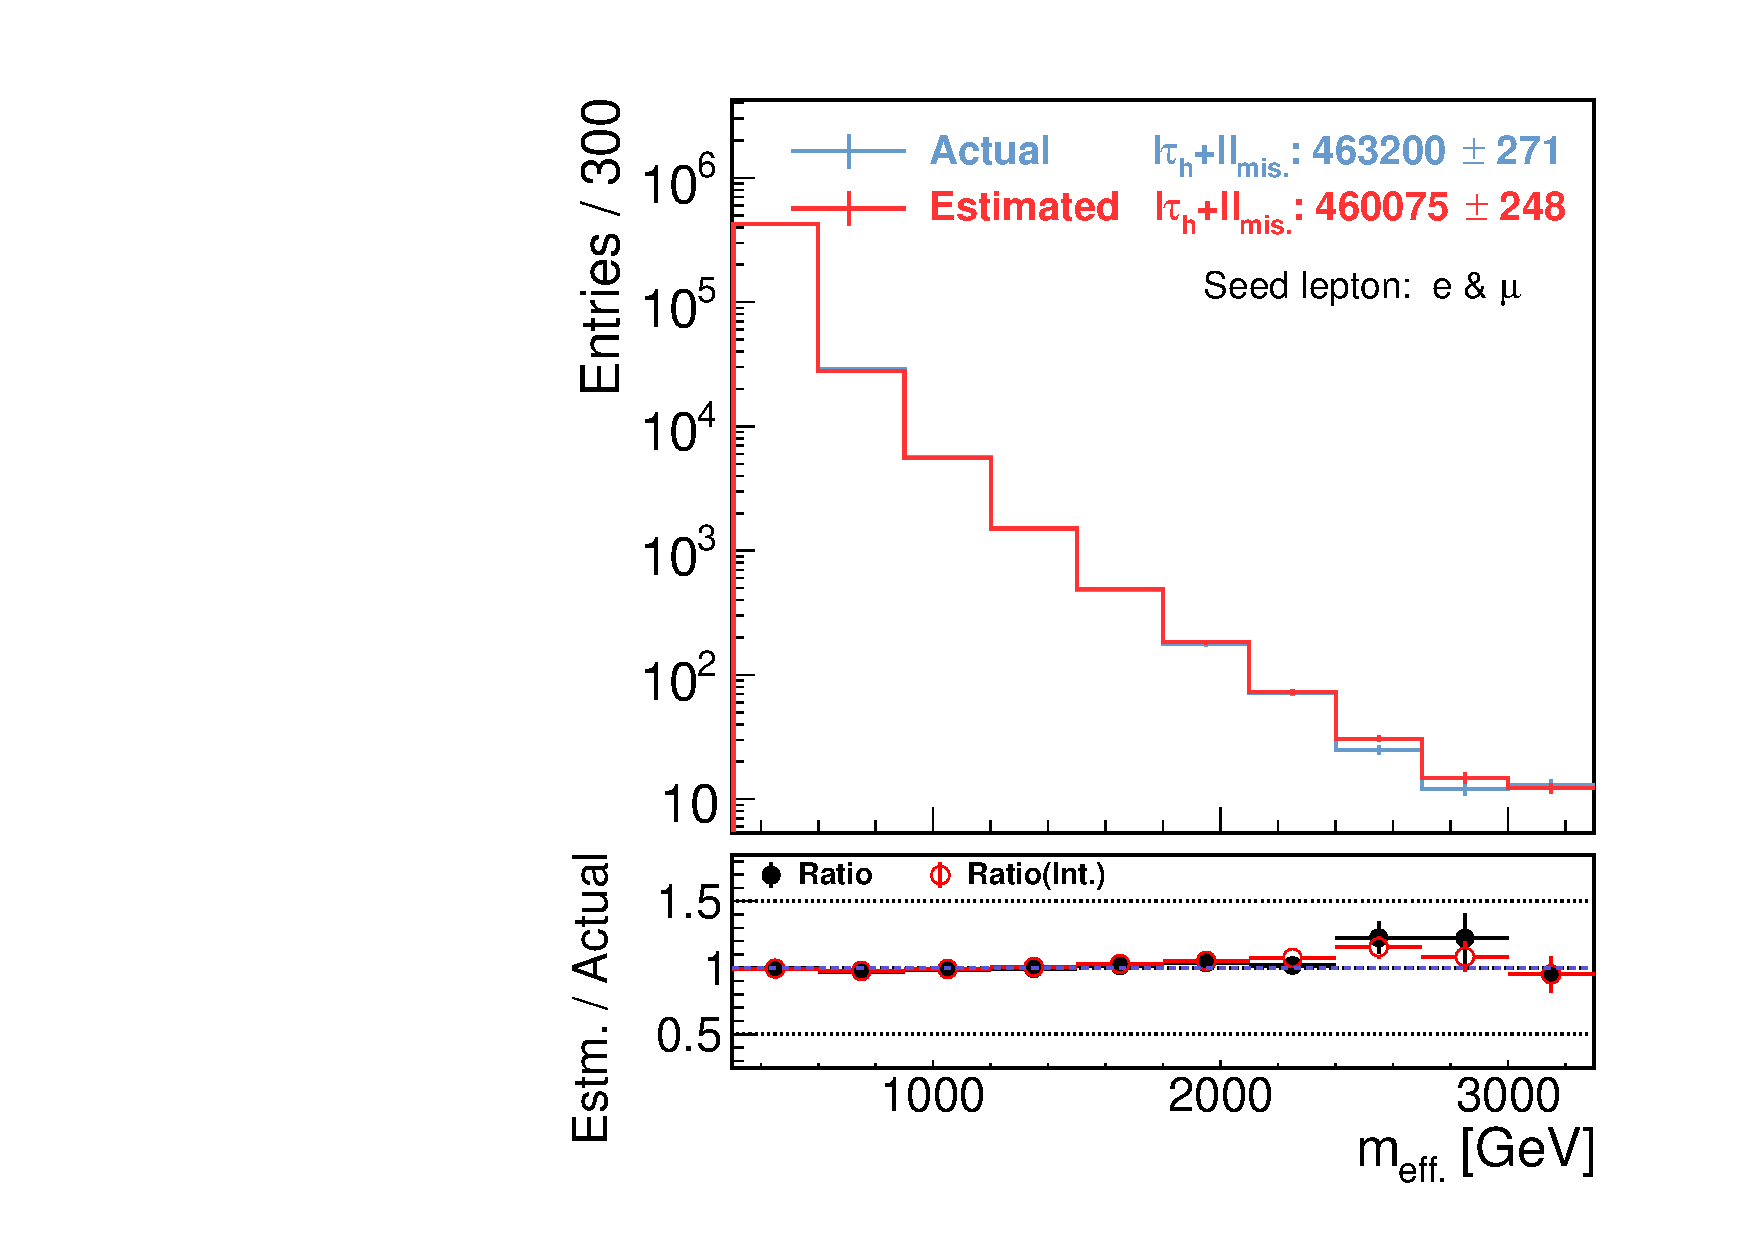
\includegraphics[width=0.32\textwidth]{figures/BGestimation/ObjReplacement/mcClosure/All_emu/All_emu_meffInc30__trMode4_NoSys.pdf}}
    \subfigure[]{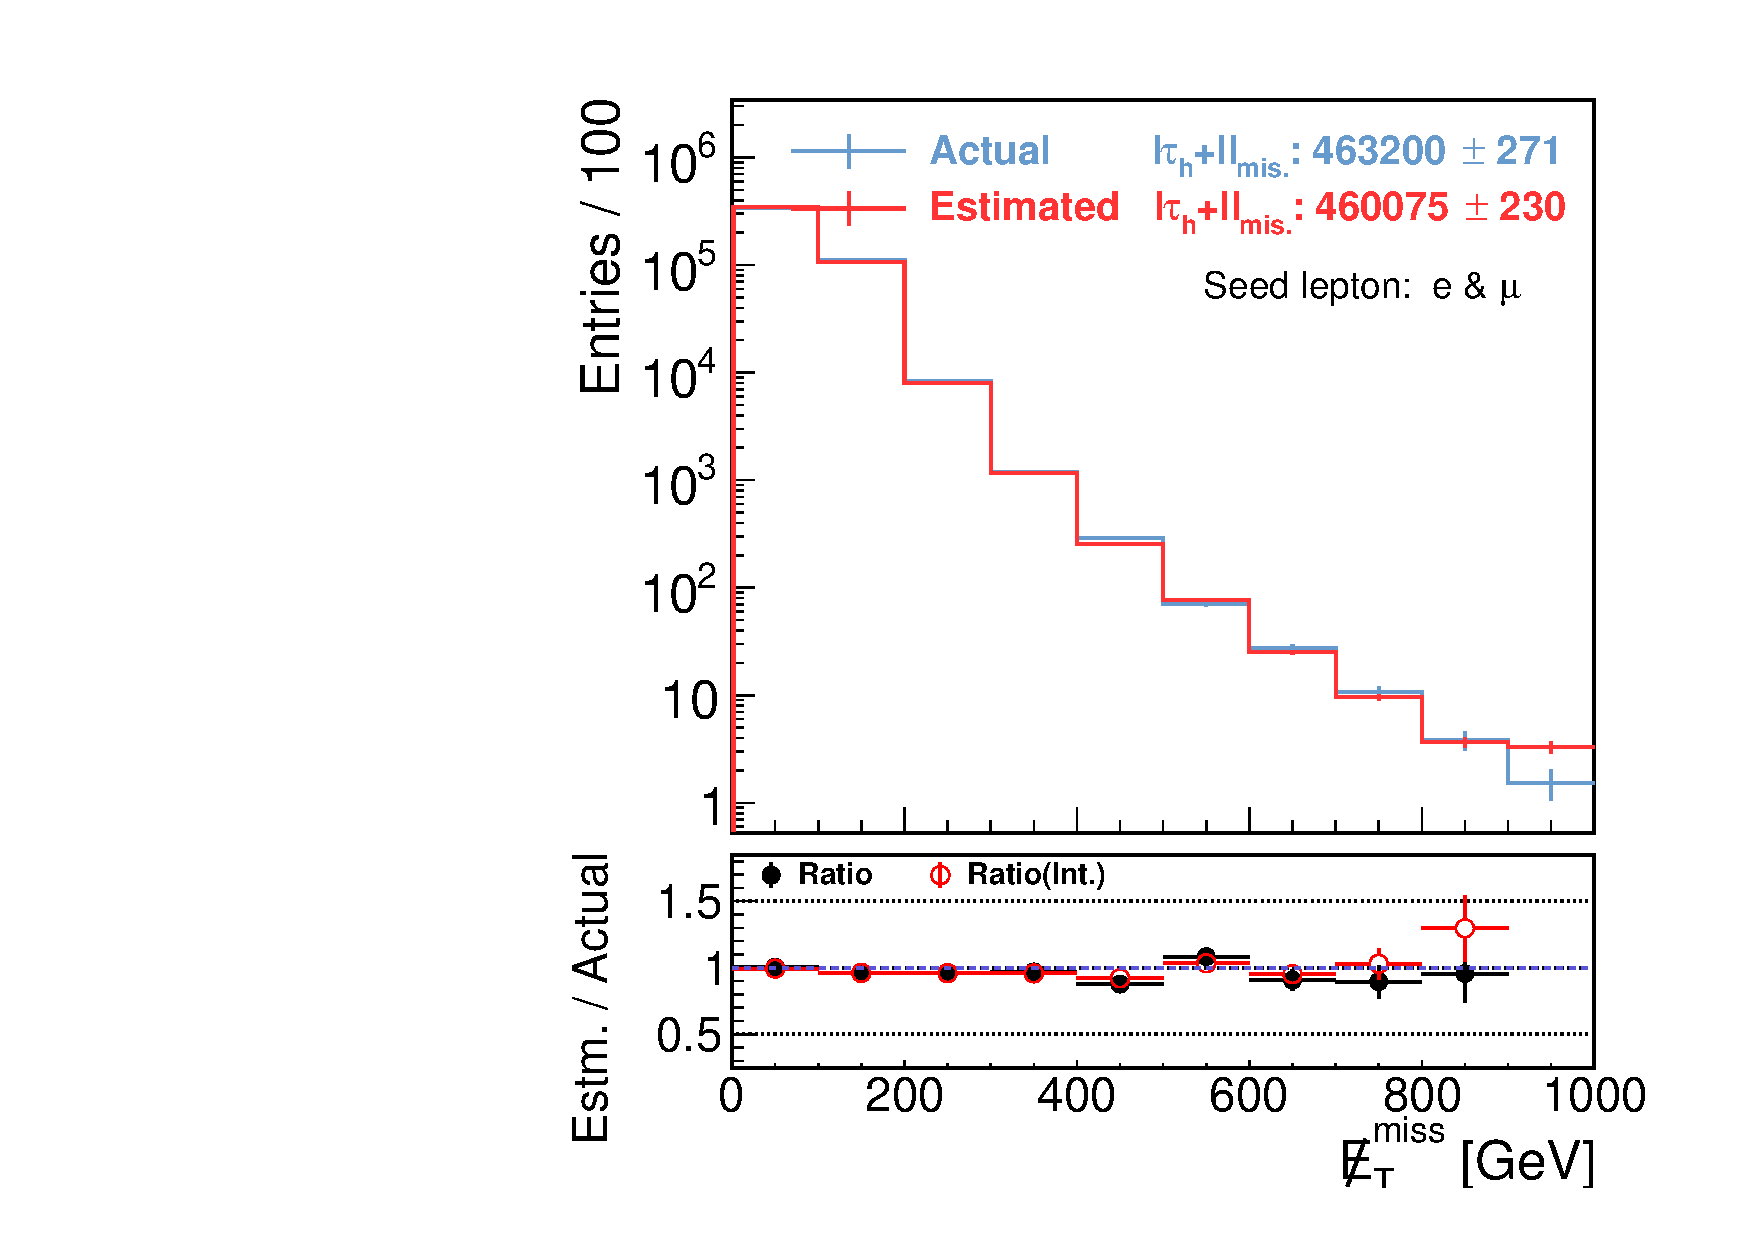
\includegraphics[width=0.32\textwidth]{figures/BGestimation/ObjReplacement/mcClosure/All_emu/All_emu_met__trMode4_NoSys.pdf}}
    \subfigure[]{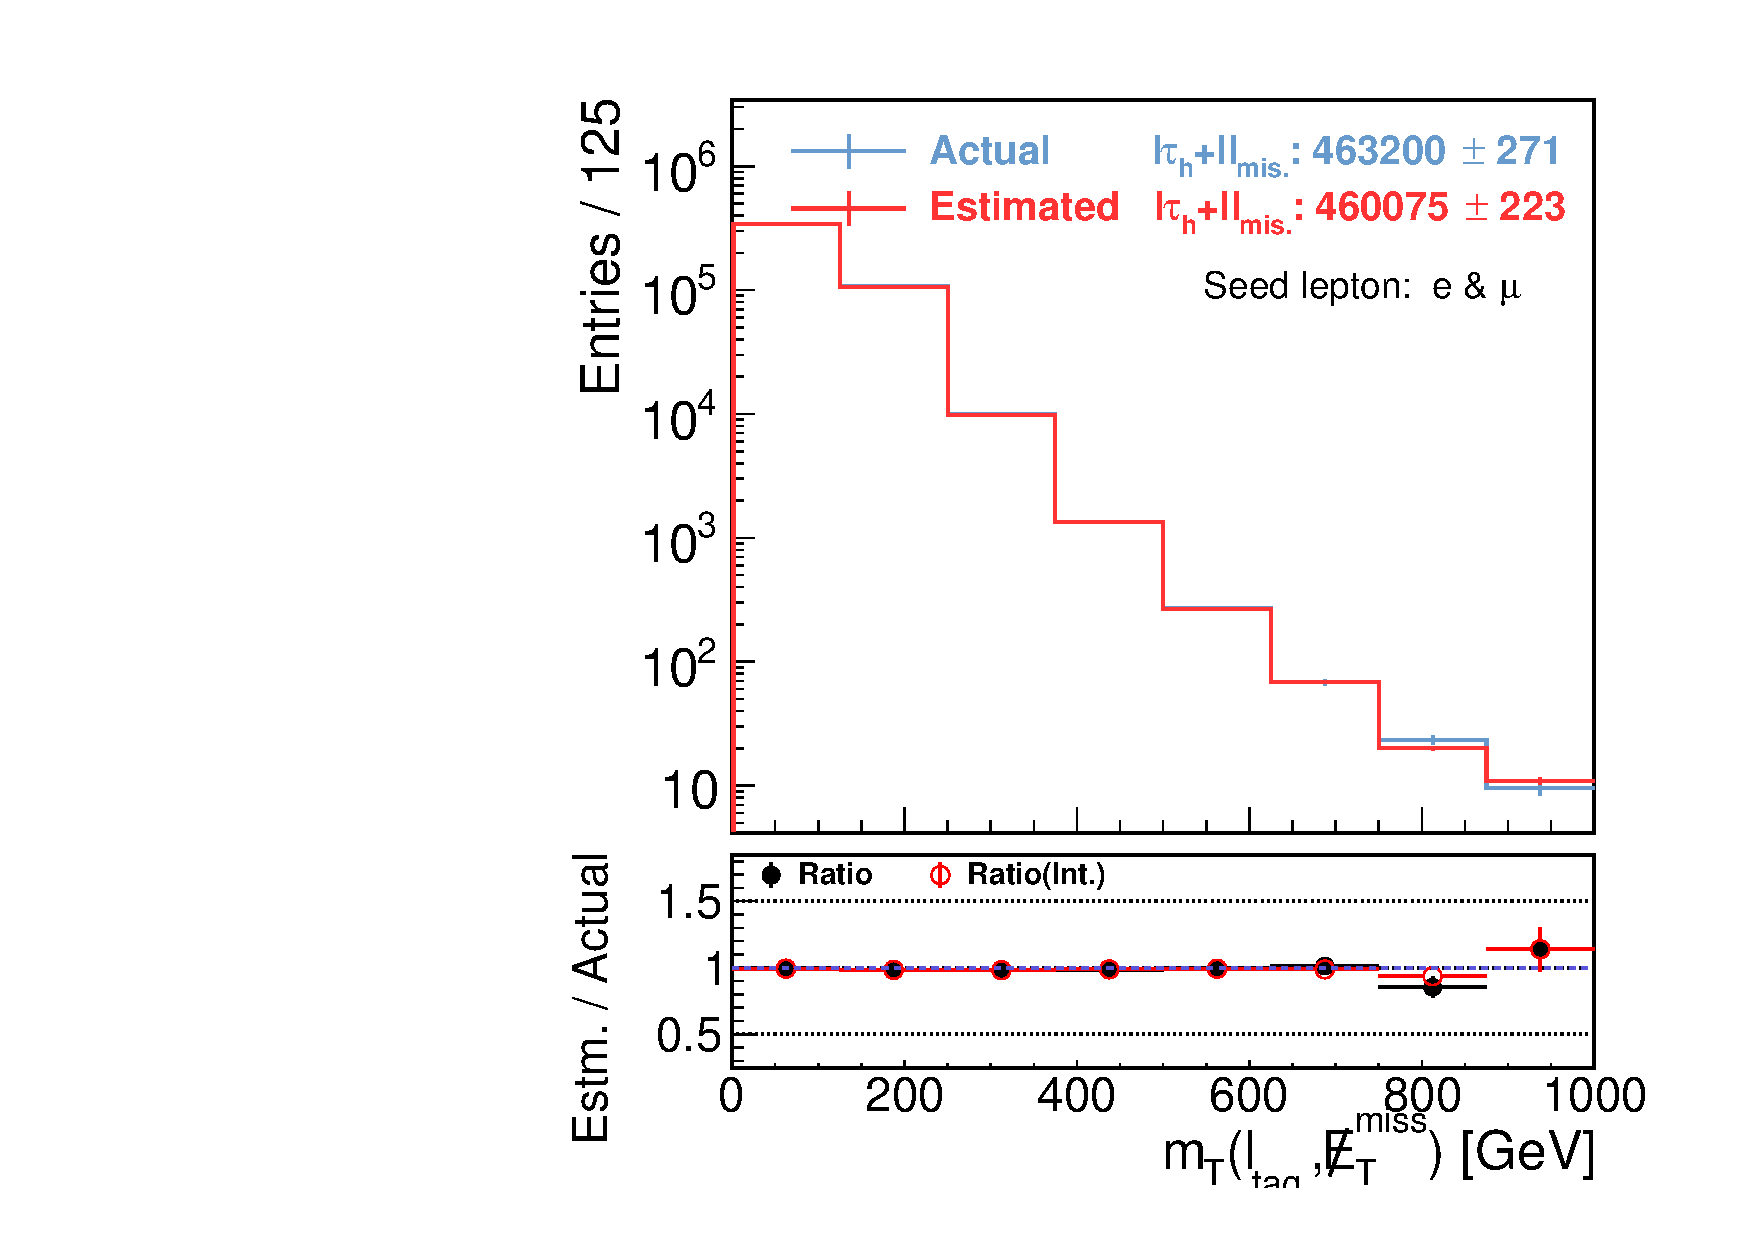
\includegraphics[width=0.32\textwidth]{figures/BGestimation/ObjReplacement/mcClosure/All_emu/All_emu_mt__trMode4_NoSys.pdf}}
    \subfigure[]{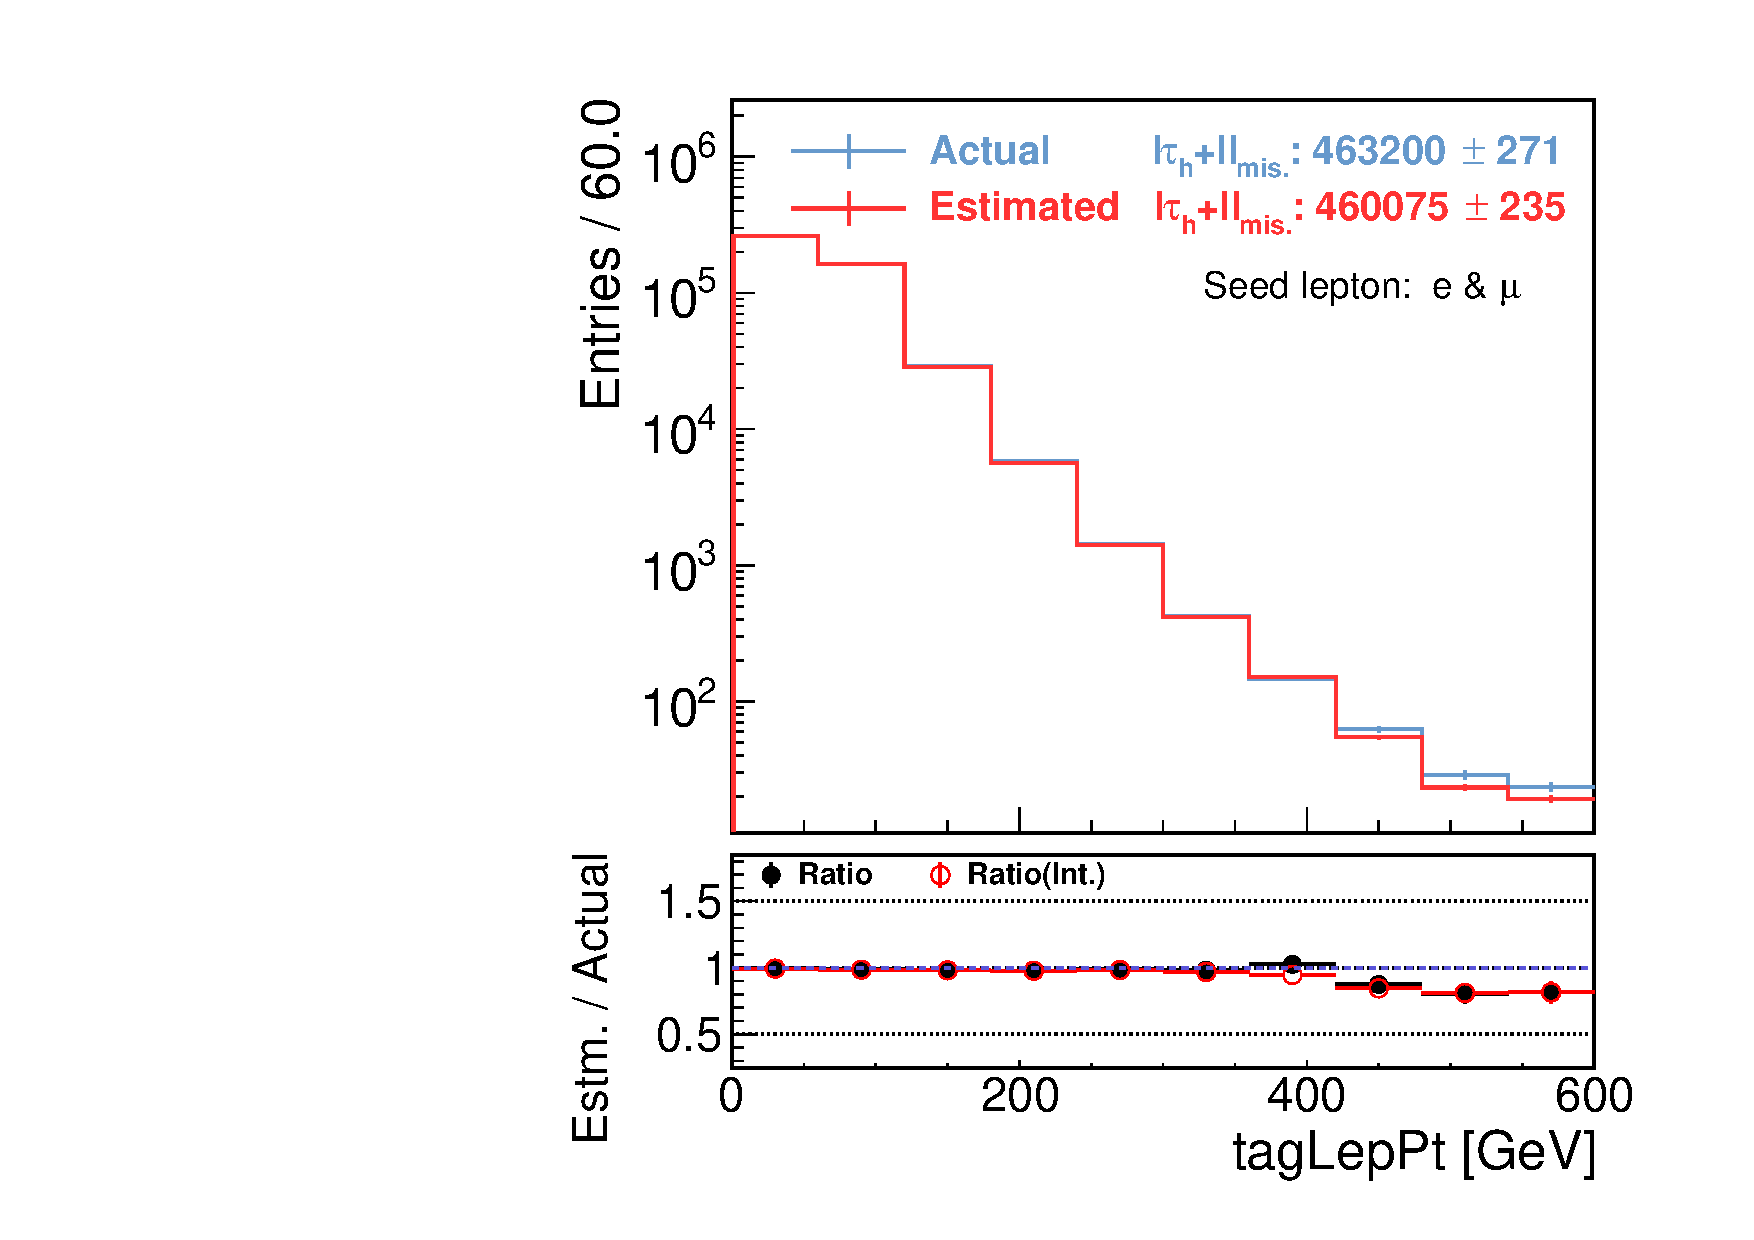
\includegraphics[width=0.32\textwidth]{figures/BGestimation/ObjReplacement/mcClosure/All_emu/All_emu_tagLepPt__trMode4_NoSys.pdf}}
    \subfigure[]{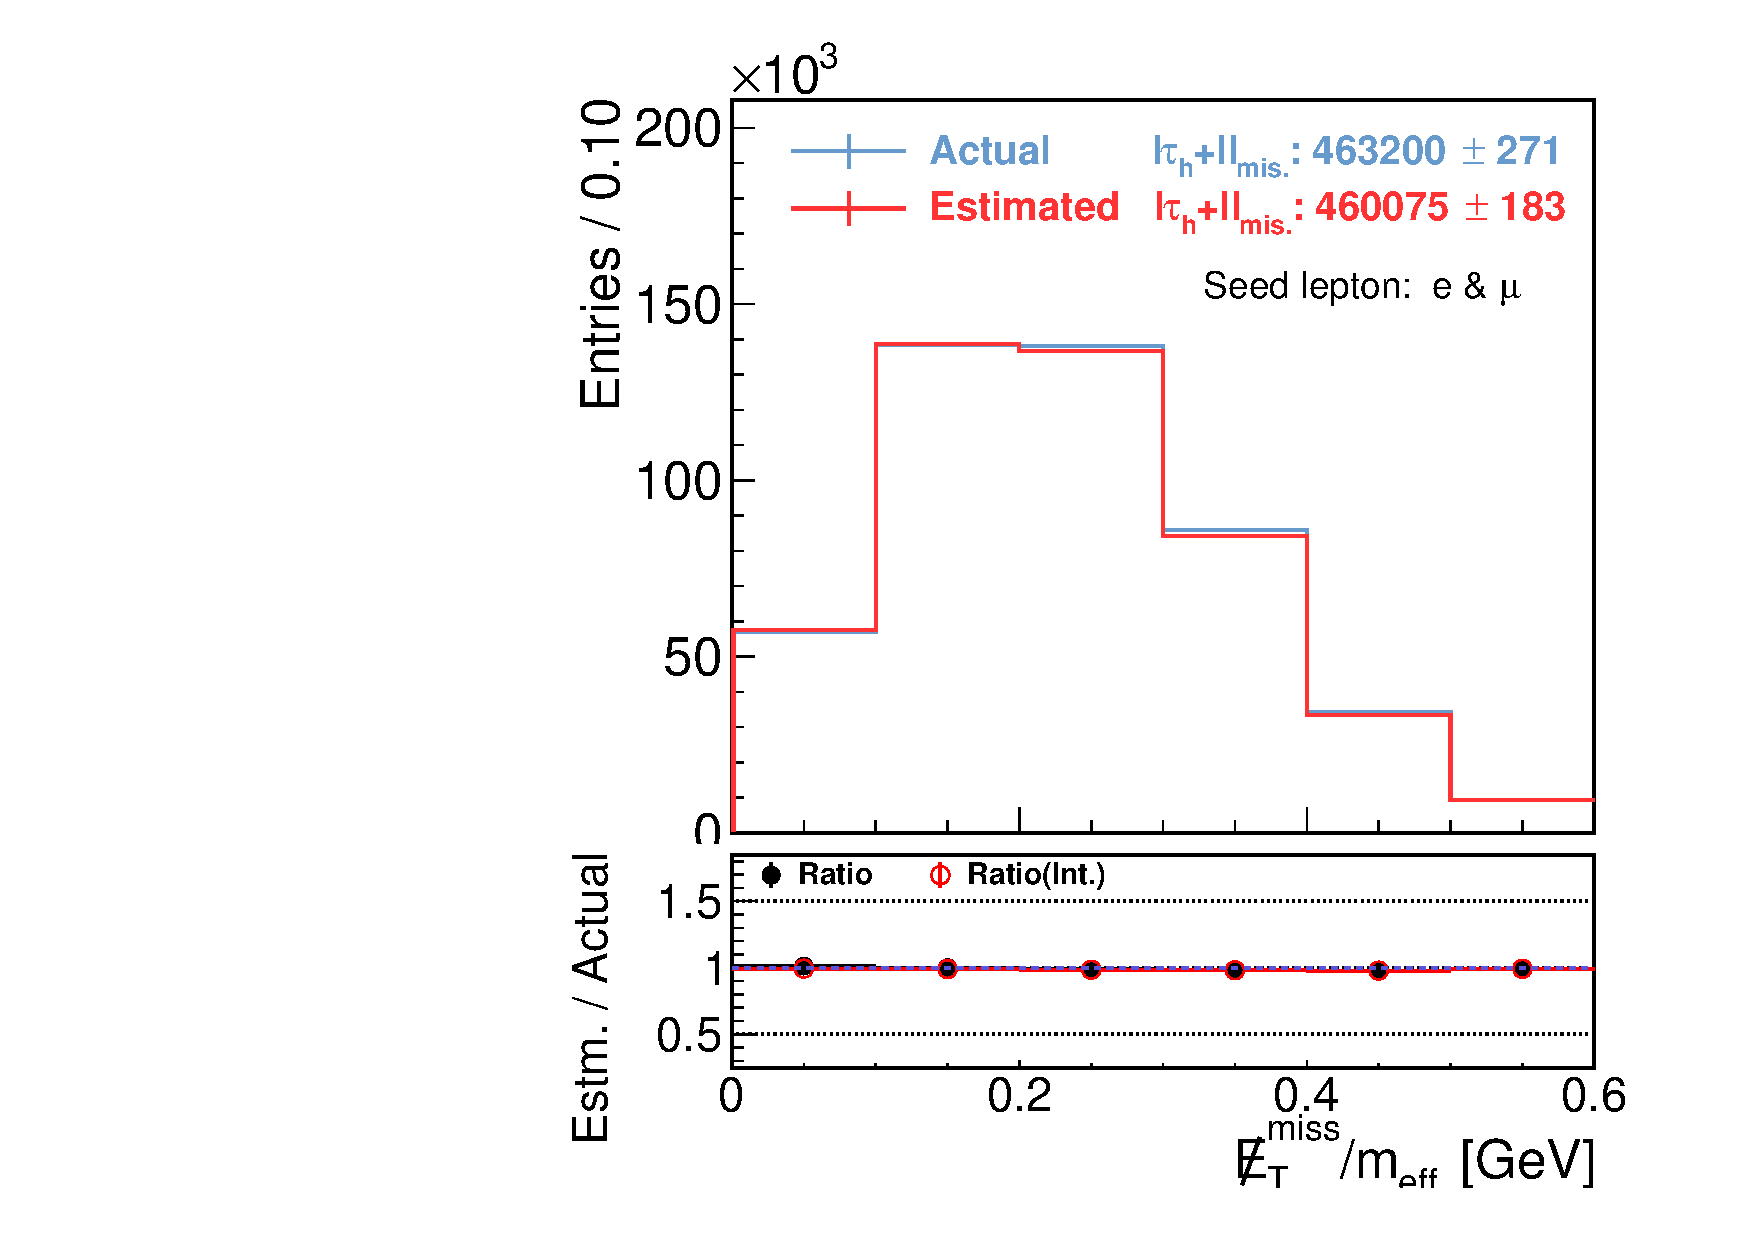
\includegraphics[width=0.32\textwidth]{figures/BGestimation/ObjReplacement/mcClosure/All_emu/All_emu_metOverMeff__trMode4_NoSys.pdf}}
    \subfigure[]{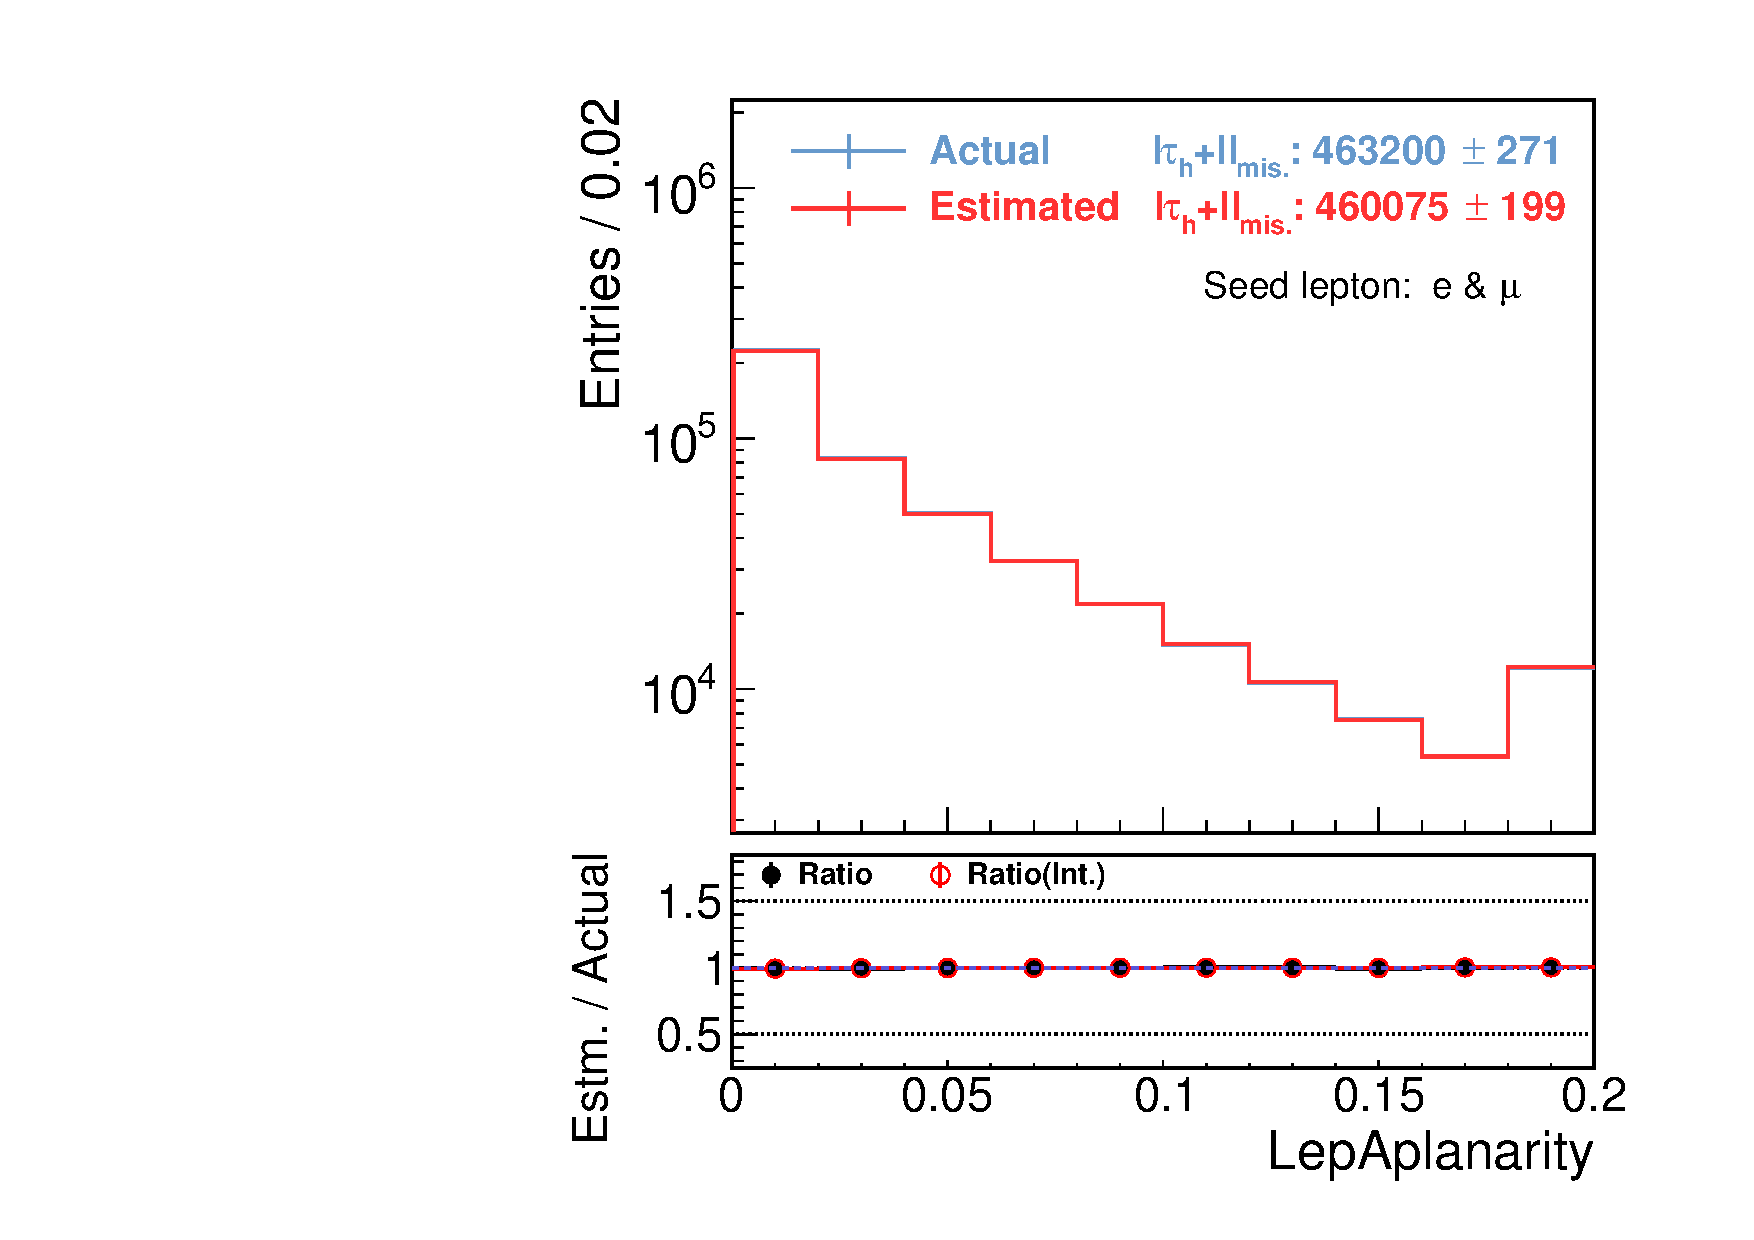
\includegraphics[width=0.32\textwidth]{figures/BGestimation/ObjReplacement/mcClosure/All_emu/All_emu_LepAplanarity__trMode4_NoSys.pdf}}
    \subfigure[]{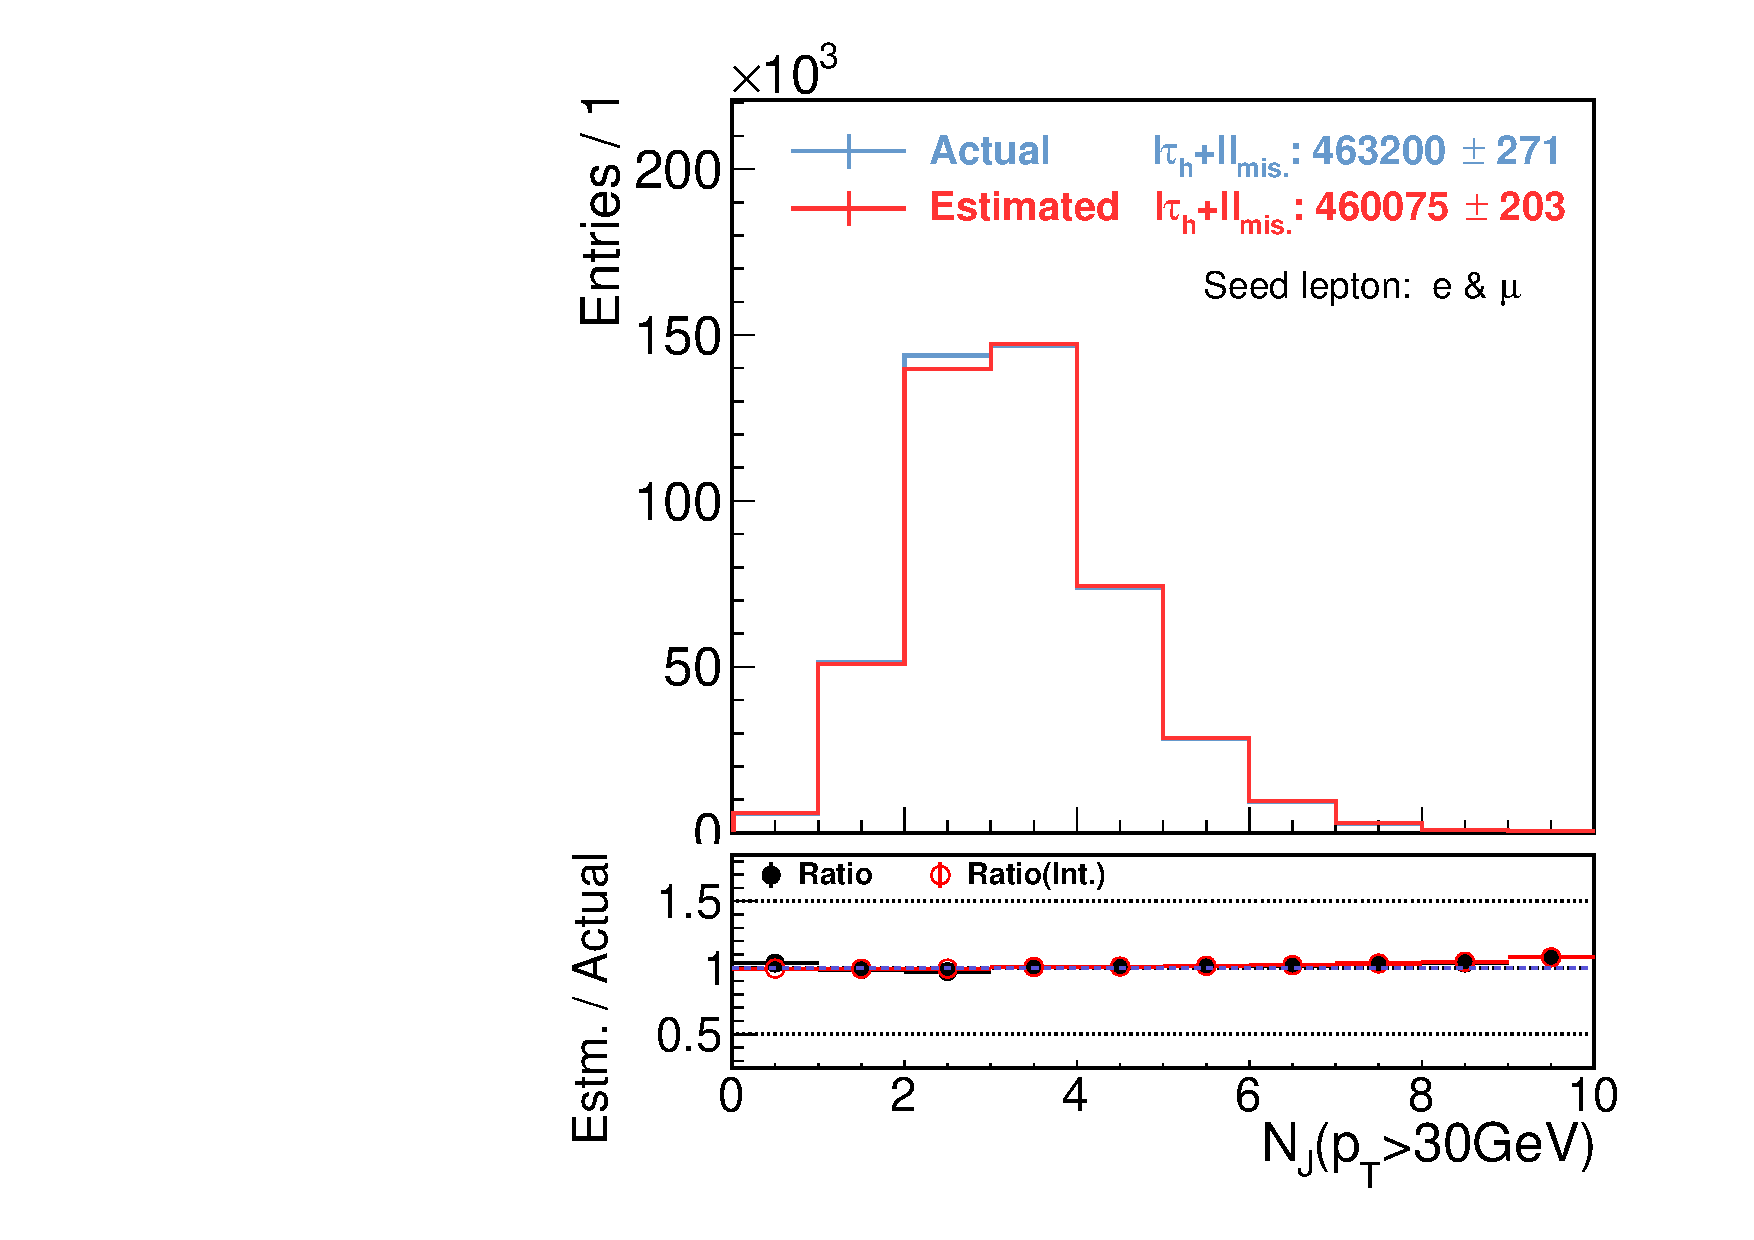
\includegraphics[width=0.32\textwidth]{figures/BGestimation/ObjReplacement/mcClosure/All_emu/All_emu_nJet30__trMode4_NoSys.pdf}}
    \subfigure[]{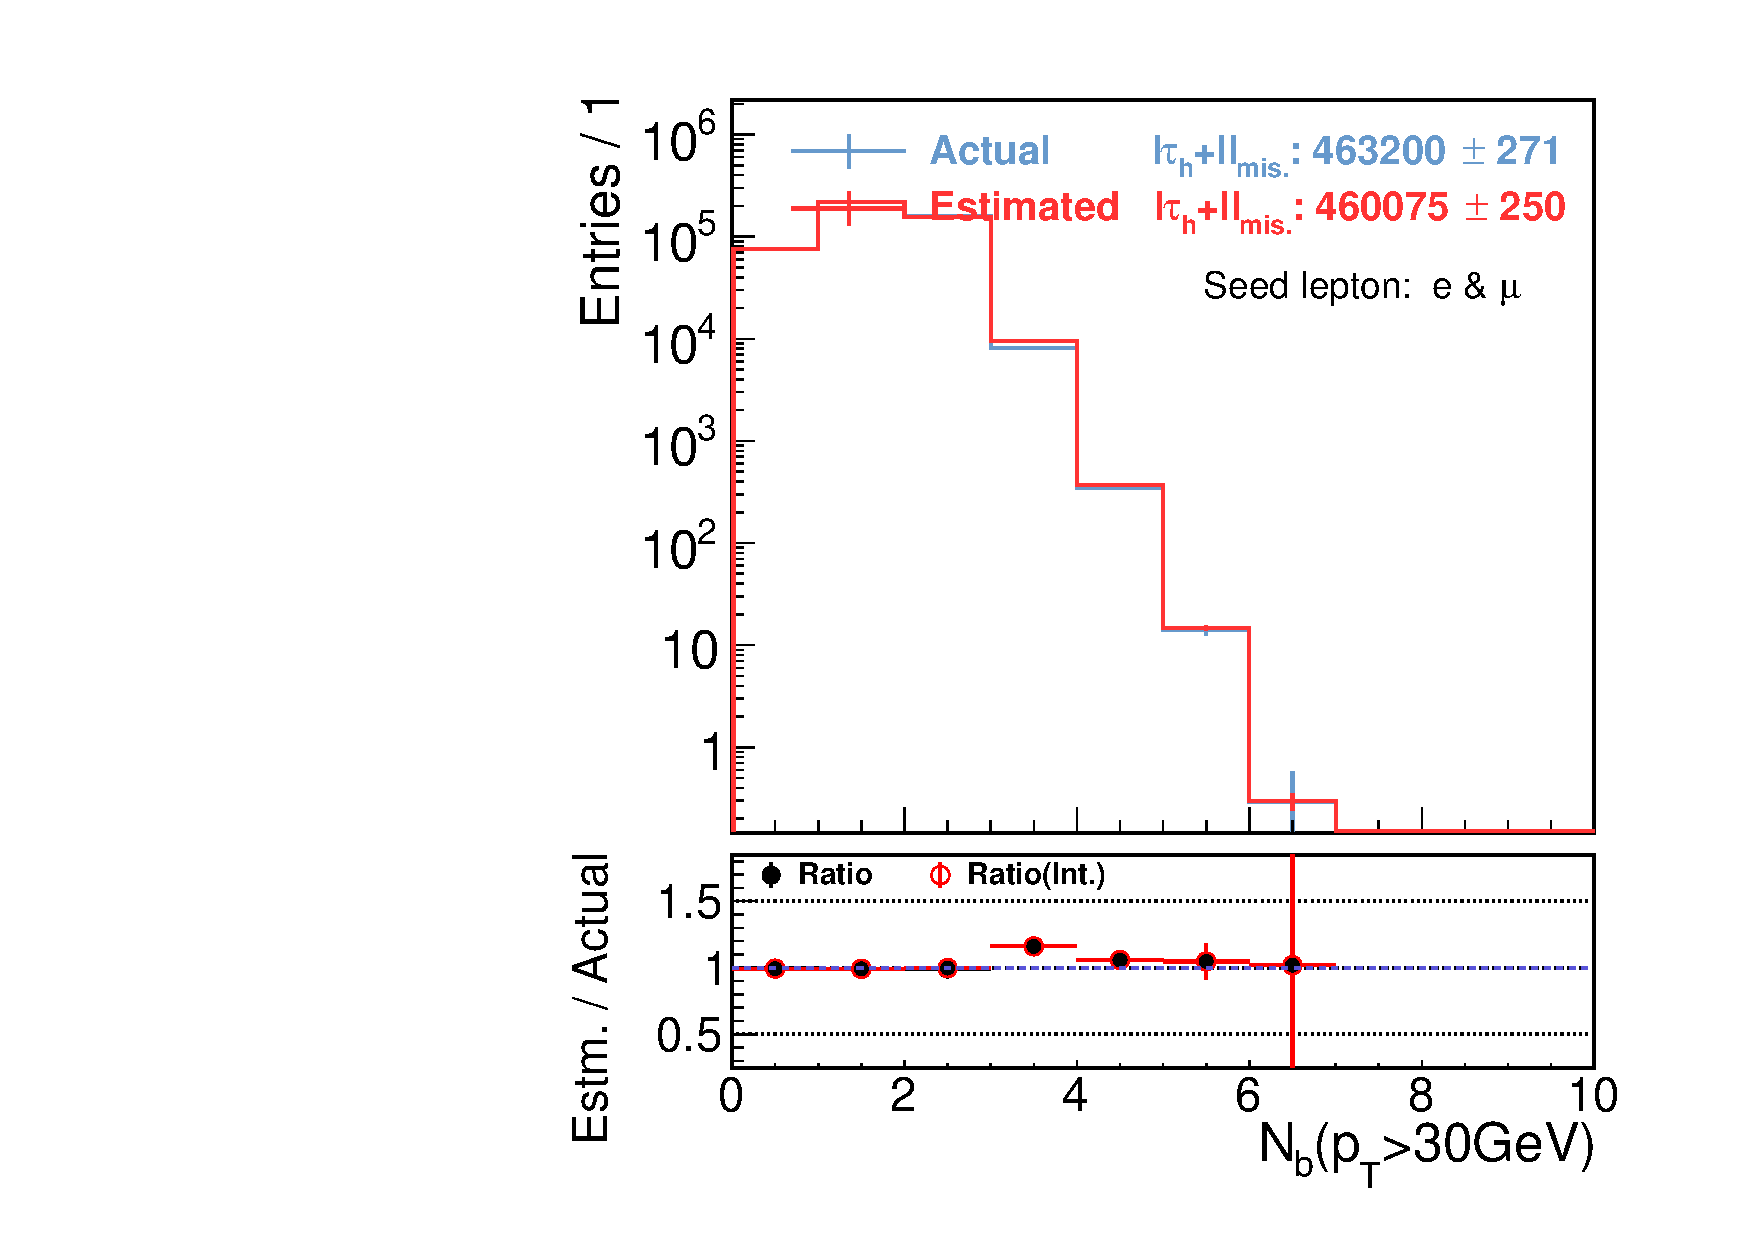
\includegraphics[width=0.32\textwidth]{figures/BGestimation/ObjReplacement/mcClosure/All_emu/All_emu_nBJet30__trMode4_NoSys.pdf}}
    \caption{ MC closure test for \textbf{combined estimation of missing lepton rep. and tau rep.} using $t\bar{t}$ MC sample. Seed events are collected by the single-lepton trigger. $p_T>35\gev$ for the leading lepton is required. \textbf{Both electrons and muons in the seed events are replaced}. Red points in the bottom plots show the ratio of integrated yields for the two histograms above the x-position that the point indicates. \label{fig::ObjReplace::mcClosure_All_emu} }
\end{figure}
 %%%%%%%%%%%%%%%%%%%%%%%%%%

